\begin{figure*}[t]
    \centering
    % \fbox{\rule{0pt}{2in} \rule{1.0\linewidth}{0pt}}
    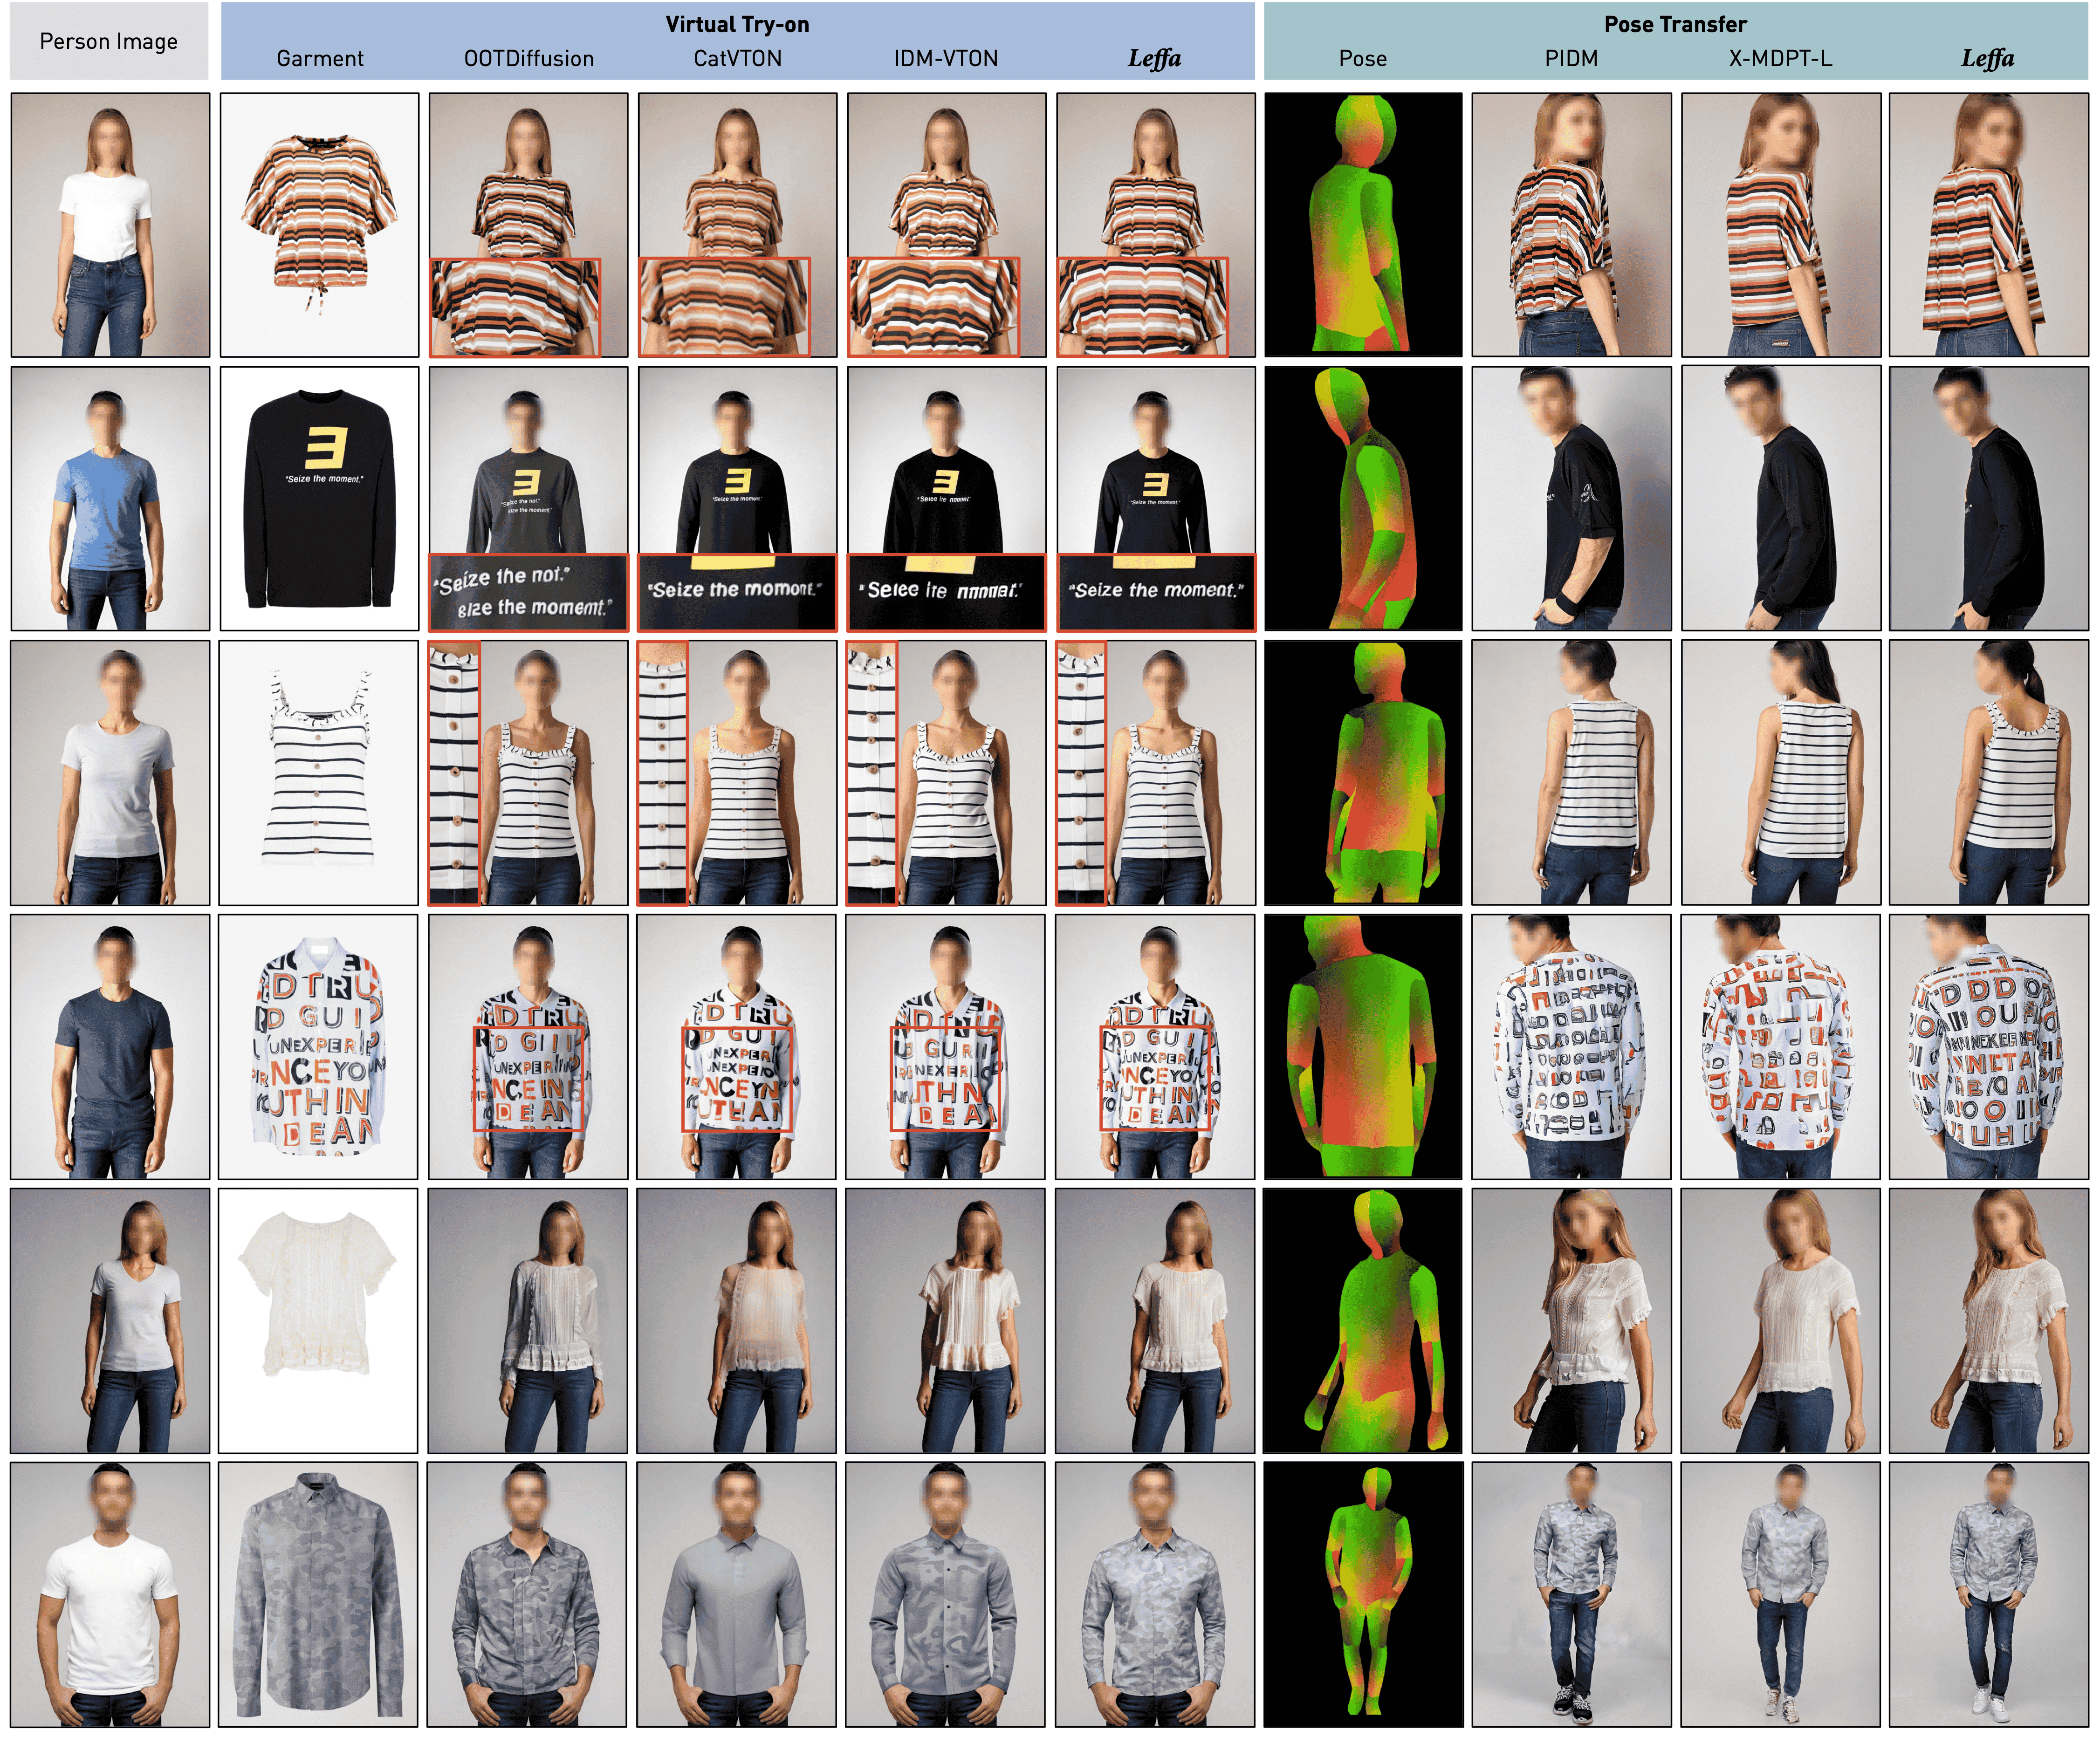
\includegraphics[width=1.0\linewidth]{Chapter6/Figures/visualization_final-min.png}
    \caption{
    Qualitative visual results comparison with other methods.
    The input person image for the pose transfer is generated using our method in the virtual try-on.
    The visualization results demonstrate that our method not only generates high-quality images but also greatly reduces the distortion of fine-grained details.
    Please zoom in for better viewing.
    }
    \label{leffa:fig:vis}
\end{figure*}


\section{Experiments}
\label{leffa:sec:exps}

\subsection{Datasets, Metrics and Implementation Details}
\label{leffa:sec:datasets}

\noindent \textbf{Datasets.}
To evaluate our method's capability in appearance and pose control, we conduct experiments on the virtual try-on and pose transfer tasks, respectively.
For virtual try-on, we use the VITON-HD~\citep{choi2021viton} and DressCode~\citep{morelli2022dress} datasets; for pose transfer, we use DeepFashion~\citep{liu2016deepfashion}. More details are provided in Appendix~D.

\noindent \textbf{Metrics.}
In virtual try-on, following previous methods~\citep{zhu2023tryondiffusion, gou2023taming, cui2023learning, cui2023street, zeng2024cat, ning2024picture, kim2024stableviton, xu2024ootdiffusion, choi2024improving, yang2024texture, chong2024catvton, yang2024d}, we evaluate the model under two settings: \textit{paired}, where the garment in the person image same as the garment image; and \textit{unpaired}, where the garments differ between the two images.
For both settings, we use FID~\citep{soloveitchik2021conditional} and KID~\citep{binkowski2018demystifying}
as evaluation metrics.
Additionally in the paired setting, we include SSIM~\citep{wang2004image} and LPIPS~\citep{zhang2018unreasonable} to evaluate image-level metrics with ground-truth data.
In pose transfer, we follow the previous methods~\citep{bhunia2023person, han2023controllable, lu2024coarse, pham2024cross} to use FID~\citep{soloveitchik2021conditional}, calculated between the generated test images and all training images; SSIM~\citep{wang2004image} and LPIPS~\citep{zhang2018unreasonable}, computed between the generated images and all images in the test set, as metrics.

\noindent \textbf{Implementation Details.}
In this chapter, we use SD1.5~\citep{rombach2022high} to build our diffusion-based baseline.
We adopt the progressive training strategy to train the model.
For virtual try-on, the model is first trained at $512 \times 384$ resolution for $10\text{k}$ steps with a batch size of 256, then at $1024 \times 768$ for $36\text{k}$ steps with a batch size of 64.
Finally, we finetune the model for an additional $10k$ steps, incorporating $\mathcal{L}_{\text{leffa}}$ to enhance its capabilities.
For pose transfer, we start at a resolution of $256 \times 176$ with a batch size of 256 for $80\text{k}$ steps, then increase to $512 \times 352$ 
for another $80\text{k}$ steps.
Finally, we finetune for $24\text{k}$ steps with $\mathcal{L}_{\text{leffa}}$.
AdamW optimizer~\citep{loshchilov2017decoupled} with a learning rate of $10^{-5}$ is applied to all training stages.
The hyperparameters for $\mathcal{L}_{\text{leffa}}$ are set as follows: $\lambda_{\text{leffa}} = 10^{-3}$, $\theta_{\text{resolution}} = 1/32$, $\theta_{\text{timestep}} = 500$ and $\tau = 2.0$.


\subsection{Quantitative and Qualitative Results}
\label{leffa:sec:main_results}

\noindent \textbf{Quantitative Comparison.}
We conduct experiments on both virtual try-on and pose transfer tasks.
For \textit{virtual try-on}, we conduct experiments on VITON-HD~\citep{choi2021viton} and DressCode~\citep{morelli2022dress}, with results shown in Tabs.~\ref{leffa:tab:viton_hd} and \ref{leffa:tab:dresscode}, respectively.
In VITON-HD, our method significantly outperforms previous methods, achieving an FID reductions of -0.88/-0.5 in the paired/unpaired setting.
In DressCode, our method also surpasses existing methods across all garment categories (upper body, lower body, and dresses), with an FID reductions of -1.93/-1.66 in the paired/unpaired setting.
% Specifically, for the upper body category, it achieves an FID reductions of -2.33 (paired) and -0.91 (unpaired); for the lower body category, -2.94 (paired) and -2.55 (unpaired); and for dresses, -1.25 (paired) and -1.71 (unpaired).
We also conduct evaluations for each garment category, with details provided in Appendix~D.
For \textit{pose transfer}, we conduct experiments on DeepFashion~\citep{liu2016deepfashion} at different resolutions, significantly outperforming previous methods.
As shown in Tab.~\ref{leffa:tab:deepfashion}, our method achieves -0.54 and -1.61 reductions in FID at $256 \times 176$ and $512 \times 352$, respectively.
While our model shows a minor SSIM gap over CFLD~\citep{lu2024coarse}, visual results and human study indicate substantial improvement over prior methods (see Fig.~\ref{leffa:fig:human_study} and Appendix~D).


\begin{table}[!t]
\centering
\setlength{\tabcolsep}{0.2cm}
\caption{Quantitative results comparison with other methods on the VITON-HD dataset for virtual try-on. Note \textbf{bold} indicates the best result, and \underline{underline} indicates the second-best result.}
\resizebox{0.8\linewidth}{!}{
\begin{tabular}{lcccccc}
\toprule[1.5pt]
\multirow{2}{*}{\textbf{Method}}        & \multicolumn{4}{c}{\textbf{paired}} & \multicolumn{2}{c}{\textbf{unpaired}} \\ \cmidrule{2-7} 
                                        & \textbf{FID} $\downarrow$ & \textbf{KID} $\downarrow$ & \textbf{SSIM} $\uparrow$ & \textbf{LPIPS} $\downarrow$ & \textbf{FID} $\downarrow$ & \textbf{KID} $\downarrow$ \\ \midrule
FS-VTON~\citep{he2022style}             & 6.17  & 0.69 & 0.886 & 0.074 & 9.91  & 1.10 \\
HR-VITON~\citep{lee2022high}            & 11.38 & 3.52 & 0.865 & 0.122 & 13.27 & 4.38 \\
GP-VTON~\citep{xie2023gp}               & 6.03  & 0.60 & 0.885 & 0.080 & 9.37  & 0.79 \\
LADI-VTON~\citep{morelli2023ladi}       & 6.60  & 1.09 & 0.866 & 0.094 & 9.35  & 1.66 \\
DCI-VTON~\citep{gou2023taming}          & 5.52  & \underline{0.41} & 0.882 & 0.080 & 8.75  & 0.68 \\
SD-VTON~\citep{shim2024towards}         & 6.98  & 1.00 & 0.874 & 0.101 & 9.85  & 1.39 \\
StableVITON~\citep{kim2024stableviton}  & 8.23  & 0.49 & \underline{0.888} & 0.073 & -     & -    \\
IDM-VTON~\citep{choi2024improving}      & 5.76  & 0.73 & 0.850 & 0.063 & 9.84  & 1.12 \\
OOTDiffusion~\citep{xu2024ootdiffusion} & 9.30  & 4.09 & 0.819 & 0.088 & 12.41 & 4.68 \\
CatVTON~\citep{chong2024catvton}        & \underline{5.42}  & \underline{0.41} & 0.870 & \underline{0.057} & \underline{9.02}  & \underline{1.09} \\
\textbf{\leffa{} (Ours)}                 & \textbf{4.54}  & \textbf{0.05} & \textbf{0.899} & \textbf{0.048} & \textbf{8.52}  & \textbf{0.32} \\
\bottomrule[1.5pt]
\end{tabular}
}
\label{leffa:tab:viton_hd}
\end{table}



\begin{table}[!t]
\centering
\setlength{\tabcolsep}{0.2cm}
\caption{Quantitative results comparison with other methods on the DressCode dataset (all garment categories) for virtual try-on. 
% Note \textbf{bold} indicates the best result, and \underline{underline} indicates the second-best result.
}
\resizebox{0.8\linewidth}{!}{
\begin{tabular}{lcccccc}
\toprule[1.5pt]
\multirow{2}{*}{\textbf{Method}}        & \multicolumn{4}{c}{\textbf{paired}} & \multicolumn{2}{c}{\textbf{unpaired}} \\ \cmidrule{2-7} 
                                        & \textbf{FID} $\downarrow$ & \textbf{KID} $\downarrow$ & \textbf{SSIM} $\uparrow$ & \textbf{LPIPS} $\downarrow$ & \textbf{FID} $\downarrow$ & \textbf{KID} $\downarrow$ \\ \midrule
% \rowcolor{tablegray} \multicolumn{7}{c}{all} \\
GP-VTON~\citep{xie2023gp}               & 9.93  & 4.61 & 0.771 & 0.180 & 12.79 & 6.63 \\
LADI-VTON~\citep{morelli2023ladi}       & 9.56  & 4.68 & 0.766 & 0.237 & 10.68 & 5.79 \\
IDM-VTON~\citep{choi2024improving}      & 6.82  & 2.92 & 0.879 & 0.056 & 9.55  & 4.32 \\
OOTDiffusion~\citep{xu2024ootdiffusion} & 4.61  & 0.96 & 0.885 & 0.053 & 12.57 & 6.63 \\
CatVTON~\citep{chong2024catvton}        & \underline{3.99}  & \underline{0.82} & \underline{0.892} & \underline{0.045} & \underline{6.14}  & \underline{1.40} \\
\textbf{\leffa{} (Ours)}                 & \textbf{2.06}  & \textbf{0.07} & \textbf{0.924} & \textbf{0.031} & \textbf{4.48} & \textbf{0.62} \\
\bottomrule[1.5pt]
\end{tabular}
}
\label{leffa:tab:dresscode}
\end{table}


\noindent \textbf{Qualitative Comparison.}
Fig.~\ref{leffa:fig:vis} shows that our method significantly improves detail preservation compared to previous methods.
For \textit{virtual try-on}, in the first row, our method accurately preserves the texture details of the colored stripes and maintains the correct color order.
In the second row, it generates very small text accurately, whereas other methods, despite achieving reasonable overall quality, exhibit varying levels of text distortion, failing to convey the correct meaning.
In the third row, our method generates evenly spaced buttons in the correct quantity, and in the fifth row, it produces a more realistic, gauzy fabric effect.
For \textit{pose transfer}, in the first to fourth rows, our method better predicts a plausible side/back-view image based on frontal information.
Other rows also show that our method maintains fine details more effectively when altering the pose.
The last row demonstrates that our method can generate vivid full-body images from half-body images.
More comparisons are provided in Appendix~D.


\begin{table}[!t]
\centering
\setlength{\tabcolsep}{0.6cm}
\caption{Quantitative results comparison with other methods on the DeepFashion dataset for pose transfer. 
% Note \textbf{bold} indicates the best result, and \underline{underline} indicates the second-best result.
}
\resizebox{0.8\linewidth}{!}{
\begin{tabular}{clccc}
\toprule[1.5pt]
\textbf{Resolution} & \textbf{Method} & \textbf{FID} $\downarrow$ & \textbf{SSIM} $\uparrow$ & \textbf{LPIPS} $\downarrow$ \\
\midrule
\multirow{13}{*}{$256 \times 176$}  & Def-GAN \citep{siarohin2018deformable} & 18.46 & 0.679 & 0.233 \\
                                    & PATN \citep{zhu2019progressive}        & 20.75 & 0.671 & 0.256 \\
                                    & ADGAN \citep{men2020controllable}      & 14.46 & 0.672 & 0.228 \\
                                    & GFLA \citep{ren2020deep}               & 10.57 & 0.707 & 0.223 \\
                                    & PISE \citep{zhang2021pise}             & 13.61 & 0.663 & 0.206 \\
                                    & DPTN \citep{zhang2022exploring}        & 11.39 & 0.711 & 0.193 \\
                                    & CASD \citep{zhou2022cross}             & 11.37 & 0.725 & 0.194 \\
                                    & NTED \citep{ren2022neural}             & 8.68  & 0.718 & 0.175 \\
                                    & PIDM \citep{bhunia2023person}          & 6.37  & 0.731 & 0.168 \\
                                    & PoCoLD \citep{han2023controllable}     & 8.07  & 0.731 & \underline{0.164} \\
                                    & CFLD \citep{lu2024coarse}              & 6.80  & \textbf{0.737} & 0.152 \\
                                    & X-MDPT-L \citep{pham2024cross}         & \underline{6.25}  & 0.729 & 0.167 \\
                                    & \textbf{\leffa{} (Ours)}               & \textbf{5.71}  &
                                    \underline{0.732} & \textbf{0.114} \\
\midrule
\multirow{8}{*}{$512 \times 352$}   & CocosNet-v2 \citep{zhou2021cocosnet}   & 13.33 & 0.724 & 0.226 \\
                                    & NTED \citep{ren2022neural}             & 7.78  & 0.738 & 0.198 \\
                                    & PIDM \citep{bhunia2023person}          & \underline{5.84}  & 0.742 & 0.177 \\
                                    & PoCoLD \citep{han2023controllable}     & 8.42  & 0.743 & 0.192 \\
                                    & CFLD \citep{lu2024coarse}              & 7.14  & \underline{0.748} & \underline{0.152} \\
                                    & X-MDPT-L \citep{pham2024cross}         & 5.93  & 0.742 & 0.179 \\
                                    & \textbf{\leffa{} (Ours)} & \textbf{4.23}  & \textbf{0.755} & \textbf{0.119} \\
% \midrule
% \multirow{1}{*}{$1024 \times 704$}  & \textbf{\leffa{} (Ours)}                         & \textbf{5.07} & \textbf{0.758} & \textbf{0.102} \\
\bottomrule[1.5pt]
\end{tabular}
}
\label{leffa:tab:deepfashion}
\end{table}


\begin{figure*}[!ht]
    \centering
    \begin{subfigure}{0.251\textwidth}
        \centering
        \resizebox{\linewidth}{!}{{% This file was created with tikzplotlib v0.10.1.
\begin{tikzpicture}

\definecolor{optiona}{RGB}{255,69,0}
\definecolor{optionb}{RGB}{138,43,226}

\begin{axis}[
width=1.61\textwidth,
height=1.2\textwidth,
ymajorgrids,
grid style=dashed,
legend columns=-1,
legend cell align={left},
legend style={
    fill=none,
    draw opacity=1,
    text opacity=1,
    at={(0.5,1.18)},
    anchor=north,
    draw=none,
    very thick,
}, 
tick align=outside,
tick pos=left,
x grid style={darkgray176},
xlabel={\large $\lambda_{leffa}$},
xmin=0, xmax=6,
xtick={0,1,2,3,4,5,6},
xticklabels={
  $0\vphantom{^{0}}$, $10^{-5}$,$10^{-4}$, $10^{-3}$, $10^{-2}$, $10^{-1}$,  $1.0\vphantom{^{0}}$
},
ylabel={FID},
ymin=4, ymax=10.5,
ytick={4,5,6,7,8,9,10},
y label style={at={(axis description cs:0.12,.5)}, anchor=south},
]
\addplot [ultra thick, optiona, mark=*, mark size=2, mark options={solid,rotate=180}]
table {%
0 5.31
1 5.2
2 4.87
3 4.54
4 5.01
5 5.57
6 6.02
};
\addlegendentry{Paired}
\addplot [ultra thick, optionb, mark=*, mark size=2, mark options={solid,rotate=180}]
table {%
0 9.38
1 9.33
2 9.02
3 8.52
4 8.97
5 9.5
6 9.97
};
\addlegendentry{Unpaired}
\end{axis}

\end{tikzpicture}
}}
        % \caption{\leffa{} loss weight}
        \label{subfig:ablation_1}
    \end{subfigure}\hfill
    \begin{subfigure}{0.249\textwidth}
        \centering
        \resizebox{\linewidth}{!}{{% This file was created with tikzplotlib v0.10.1.
\begin{tikzpicture}

\definecolor{optiona}{RGB}{255,69,0}
\definecolor{optionb}{RGB}{138,43,226}

\begin{axis}[
width=1.54\textwidth,
height=1.2\textwidth,
ymajorgrids,
grid style=dashed,
legend columns=-1,
legend cell align={left},
legend style={
    fill=none,
    draw opacity=1,
    text opacity=1,
    at={(0.5,1.18)},
    anchor=north,
    draw=none,
    very thick,
}, 
tick align=outside,
tick pos=left,
x grid style={darkgray176},
xlabel={\large $\theta_{resolution}$},
xmin=0, xmax=3,
xtick style={color=black},
xtick={0,1,2,3},
xticklabels={1/8,1/16,1/32,1/64},
ylabel={FID},
ymin=4, ymax=10.5,
ytick={4,5,6,7,8,9,10},
y label style={at={(axis description cs:0.12,.5)}, anchor=south},
]
\addplot [ultra thick, optiona, mark=*, mark size=2, mark options={solid,rotate=180}]
table {%
0 5.03
1 4.67
2 4.59
3 5.22
};
\addlegendentry{Paired}
\addplot [ultra thick, optionb, mark=*, mark size=2, mark options={solid,rotate=180}]
table {%
0 9.17
1 8.66
2 8.54
3 9.3
};
\addlegendentry{Unpaired}
\end{axis}

\end{tikzpicture}
}}
        % \caption{resolution threshold}
        \label{subfig:ablation_2}
    \end{subfigure}\hfill
    \begin{subfigure}{0.249\textwidth}
        \centering
        \resizebox{\linewidth}{!}{{% This file was created with tikzplotlib v0.10.1.
\begin{tikzpicture}

\definecolor{optiona}{RGB}{255,69,0}
\definecolor{optionb}{RGB}{138,43,226}

\begin{axis}[
width=1.55\textwidth,
height=1.2\textwidth,
ymajorgrids,
grid style=dashed,
legend columns=-1,
legend cell align={left},
legend style={
    fill=none,
    draw opacity=1,
    text opacity=1,
    at={(0.5,1.18)},
    anchor=north,
    draw=none,
    very thick,
}, 
tick align=outside,
tick pos=left,
xlabel={\large $\theta_{timestep}$},
xmin=0, xmax=3,
xtick={0,1,2,3},
xticklabels={250,500,750,1000},
ylabel={FID},
ymin=4, ymax=10.5,
ytick={4,5,6,7,8,9,10},
y label style={at={(axis description cs:0.12,.5)}, anchor=south},
]
\addplot [ultra thick, optiona, mark=*, mark size=2, mark options={solid,rotate=180}]
table {%
0 4.74
1 4.59
2 5.1
3 5.73
};
\addlegendentry{Paired}
\addplot [ultra thick, optionb, mark=*, mark size=2, mark options={solid,rotate=180}]
table {%
0 8.83
1 8.54
2 9.22
3 9.53
};
\addlegendentry{Unpaired}
\end{axis}

\end{tikzpicture}
}}
        % \caption{timestep threshold}
        \label{subfig:ablation_3}
    \end{subfigure}\hfill
    \begin{subfigure}{0.249\textwidth}
        \centering
        \resizebox{\linewidth}{!}{{% This file was created with tikzplotlib v0.10.1.
\begin{tikzpicture}

\definecolor{optiona}{RGB}{255,69,0}
\definecolor{optionb}{RGB}{138,43,226}

\begin{axis}[
width=1.56\textwidth,
height=1.2\textwidth,
ymajorgrids,
grid style=dashed,
legend columns=-1,
legend cell align={left},
legend style={
    fill=none,
    draw opacity=1,
    text opacity=1,
    at={(0.5,1.18)},
    anchor=north,
    draw=none,
    very thick,
}, 
tick align=outside,
tick pos=left,
x grid style={darkgray176},
xlabel={\large temperature $\tau$},
xmin=0, xmax=4,
xtick={0,1,2,3,4},
xticklabels={0.1,0.5,1.0,2.0,5.0},
ylabel={FID},
ymin=4, ymax=10.5,
ytick={4,5,6,7,8,9,10},
y label style={at={(axis description cs:0.12,.5)}, anchor=south},
]
\addplot [ultra thick, optiona, mark=*, mark size=2, mark options={solid,rotate=180}]
table {%
0 5.46
1 4.8
2 4.71
3 4.59
4 5.48
};
\addlegendentry{Paired}
\addplot [ultra thick, optionb, mark=*, mark size=2, mark options={solid,rotate=180}]
table {%
0 9.94
1 8.85
2 8.78
3 8.54
4 9.32
};
\addlegendentry{Unpaired}
\end{axis}

\end{tikzpicture}
}}
        % \caption{temperature threshold}
        \label{subfig:ablation_4}
    \end{subfigure}
    \caption{Ablation study for (a) \leffa{} loss weight $\lambda_{\text{leffa}}$, (b) resolution threshold $\theta_{\text{resolution}}$, (c) timestep threshold $\theta_{\text{timestep}}$, (d) temperature $\tau$ on VITON-HD dataset of virtual try-on.}
    \label{leffa:fig:ablation}
\end{figure*}


\begin{figure}[t]
    \centering
    % \fbox{\rule{0pt}{2in} \rule{1.0\linewidth}{0pt}}
    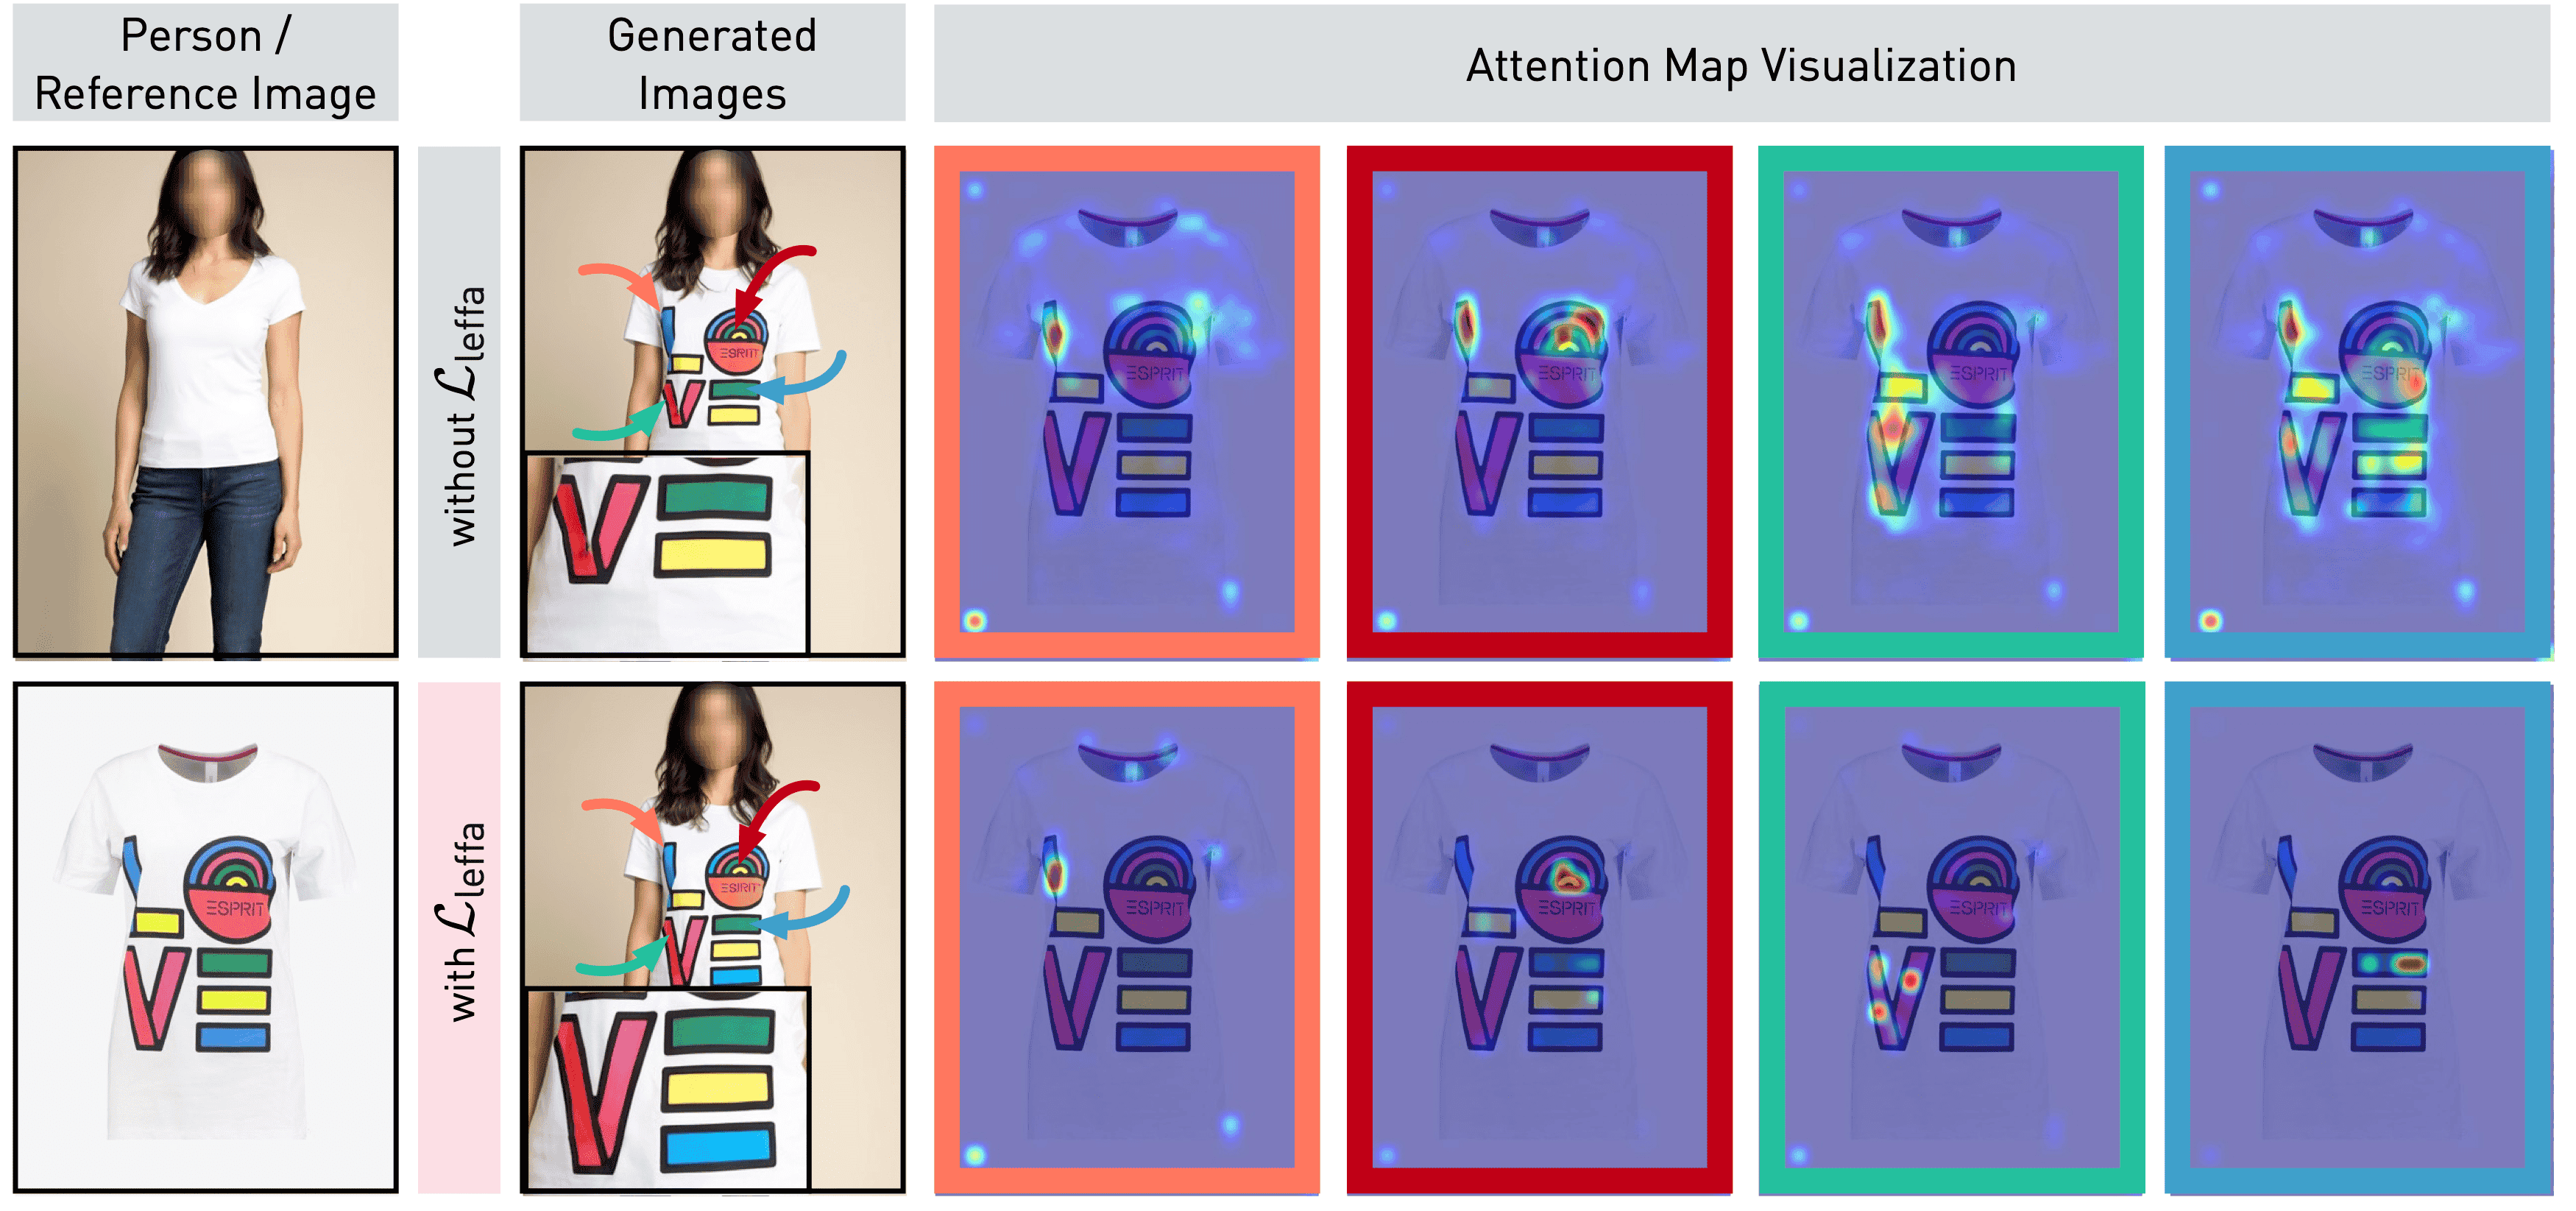
\includegraphics[width=1.0\linewidth]{Chapter6/Figures/vis_ablation_final-min.png}
    \caption{
    Visualization of feature maps to assess the impact of our \leffa{} loss $\mathcal{L}_\text{leffa}$.
    With our \leffa{} loss added, our method not only maintains overall generation quality but also more accurately preserves fine-grained details.
    Additionally, attention map visualizations indicate that, with our loss, the target query focuses more precisely on the correct reference region.
    }
    \label{leffa:fig:vis_ablation}
\end{figure}


\subsection{Generalization to Other Diffusion Models}

The proposed \leffa{} loss is model-agnostic and can be applied to different attention-based methods.
We evaluate this by adding \leffa{} loss to two prior art diffusion-based methods (\ie, IDM-VTON~\citep{choi2024improving} and CatVTON~\citep{chong2024catvton}) on the VITON-HD~\citep{choi2021viton} dataset.
Since both methods also use attention mechanism to interact with the reference image, our \leffa{} loss can be seamlessly integrated without introducing extra trainable parameters.
As shown in Tab.~\ref{leffa:tab:general}, our method achieves FID reductions of -0.64/-0.6 for IDM-VTON and -0.56/-0.25 for CatVTON in paired/unpaired settings, confirming its generalization ability.


\begin{table}[!t]
\centering
\setlength{\tabcolsep}{0.3cm}
\caption{Applying our \leffa{} loss $\mathcal{L}_\text{leffa}$ consistently enhances performance across different diffusion-based methods.}
\resizebox{0.8\linewidth}{!}{
\begin{tabular}{lccccccc}
\toprule[1.5pt]
\multirow{2}{*}{\textbf{Method}}  & \multirow{2}{*}{\textbf{$\mathcal{L}_{\text{leffa}}$}}        & \multicolumn{4}{c}{\textbf{paired}} & \multicolumn{2}{c}{\textbf{unpaired}} \\ \cmidrule{3-8} 
                                        & & \textbf{FID} $\downarrow$ & \textbf{KID} $\downarrow$ & \textbf{SSIM} $\uparrow$ & \textbf{LPIPS} $\downarrow$ & \textbf{FID} $\downarrow$ & \textbf{KID} $\downarrow$ \\ 
\midrule
\multirow{2}{*}{IDM-VTON}   & \xmark          & 5.76  & 0.73 & 0.850 & 0.063 & 9.84  & 1.12 \\ 
  & \cmark & 5.12 & 0.35 & 0.876 & 0.054 & 9.24 & 0.87 \\ \midrule[0.5pt]
\multirow{2}{*}{CatVTON}   & \xmark          & 5.42  & 0.41 & 0.870 & 0.057 & 9.02  & 1.09 \\
   & \cmark & 4.86 & 0.28 & 0.886 & 0.056 & 8.77 & 0.58 \\ \midrule[0.5pt]
\multirow{2}{*}{Ours}     & \xmark          & 5.31  & 0.30 & 0.885 & 0.058 & 9.38  & 0.91 \\
      & \cmark & \textbf{4.54}  & \textbf{0.05} & \textbf{0.899} & \textbf{0.048} & \textbf{8.52}  & \textbf{0.32} \\
\bottomrule[1.5pt]
\end{tabular}
}
\label{leffa:tab:general}
\end{table}


\subsection{Ablation Study}
\label{leffa:sec:ablation}

To further validate the effectiveness of our method, we conduct ablation experiments on the VITON-HD dataset.

\noindent \textbf{Effect of $\mathcal{L}_{\text{leffa}}$}.
We first ablate \leffa{} loss to evaluate the benefits of learning flow fields in attention.
As shown in Tab.~\ref{leffa:tab:general}, all metrics degrade without $\mathcal{L}_{\text{leffa}}$.
Specifically, the FID worsens by +0.77/+0.86 in the paired/unpaired setting, clearly demonstrating the contribution of our \leffa{} loss to improving overall generation quality.
We further present visualizations of attention maps using \leffa{} in Fig.~\ref{leffa:fig:vis_ablation}, which clearly show that the attended regions (highlighted in red) accurately correspond to the desired reference regions.

We additionally conduct a list of ablations to search the optimal training hyperparameters for our \leffa{} loss.

\noindent \textbf{Effect of Different $\lambda_{\text{leffa}}$.} 
In Fig.~\ref{leffa:fig:ablation}, we find that by increasing $\lambda_{\text{leffa}}$ from $0.0$ to $10^{-3}$ improves performance, but further increasing to a degradation in performance.
This suggests that while the \leffa{} loss effectively guides attention, overly strong supervision can hinder generalization, ultimately degrading generation quality.

% \begin{table}[!t]
% \centering
% \resizebox{0.85\linewidth}{!}{
% \begin{tabular}{lcccccc}
% \toprule[1.5pt]
% \multirow{2}{*}{\textbf{$\lambda_{\text{leffa}}$}}        & \multicolumn{4}{c}{\textbf{paired}} & \multicolumn{2}{c}{\textbf{unpaired}} \\ \cmidrule{2-7} 
%                                         & \textbf{FID} $\downarrow$ & \textbf{KID} $\downarrow$ & \textbf{SSIM} $\uparrow$ & \textbf{LPIPS} $\downarrow$ & \textbf{FID} $\downarrow$ & \textbf{KID} $\downarrow$ \\ \midrule
% $0.0$                                   & 5.31  & 0.30 & 0.885 & 0.058 & 9.38  & 0.91 \\
% $10^{-5}$                               & 5.20 & 0.31 & 0.886 & 0.058 & 9.33 & 0.90 \\
% $10^{-4}$                               & 4.87 & 0.25 & 0.889 & 0.057 & 9.02 & 0.78 \\
% $10^{-3}$                               & \textbf{4.59}  & \textbf{0.10} & \textbf{0.893} & \textbf{0.052} & \textbf{8.54}  & \textbf{0.44} \\
% $10^{-2}$                               & 5.01 & 0.28 & 0.892 & 0.055 & 8.97 & 0.82 \\
% $10^{-1}$                               & 5.57 & 0.40 & 0.885 & 0.061 & 9.50 & 0.95 \\
% $1.0$                                   & 6.02 & 0.83 & 0.880 & 0.082 & 9.97 & 1.22 \\
% \bottomrule[1.5pt]
% \end{tabular}
% }
% \caption{Ablation study for \leffa{} loss weight $\lambda_{\text{leffa}}$.}
% \label{leffa:tab:lambda_flow}
% \end{table}


\noindent \textbf{Effect of Resolution Threshold $\theta_{\text{resolution}}$.}
In Fig.~\ref{leffa:fig:ablation}, we observe that the optimal performance appears when $\theta_{\text{resolution}}$ is within $1/32$ and $1/16$.
Otherwise, attention maps are either too large (resulting in too few attention layers) or too small to focus on the correct regions.

% \begin{table}[!t]
% \centering
% \resizebox{0.85\linewidth}{!}{
% \begin{tabular}{lcccccc}
% \toprule[1.5pt]
% \multirow{2}{*}{\textbf{$\theta_{\text{resolution}}$}}        & \multicolumn{4}{c}{\textbf{paired}} & \multicolumn{2}{c}{\textbf{unpaired}} \\ \cmidrule{2-7} 
%                                         & \textbf{FID} $\downarrow$ & \textbf{KID} $\downarrow$ & \textbf{SSIM} $\uparrow$ & \textbf{LPIPS} $\downarrow$ & \textbf{FID} $\downarrow$ & \textbf{KID} $\downarrow$ \\ \midrule
% 1/8                                     & 5.03 & 0.28 & 0.886 & 0.063 & 9.17 & 0.61 \\
% 1/16                                    & 4.67 & 0.14 & \textbf{0.895} & \textbf{0.052} & 8.66 & 0.52 \\
% 1/32                                    & \textbf{4.59}  & \textbf{0.10} & 0.893 & \textbf{0.052} & \textbf{8.54}  & \textbf{0.44} \\
% 1/64                                    & 5.22 & 0.34 & 0.885 & 0.057 & 9.30 & 1.01 \\
% \bottomrule[1.5pt]
% \end{tabular}
% }
% \caption{Ablation study for resolution threshold $\theta_{\text{resolution}}$.}
% \label{leffa:tab:theta_resolution}
% \end{table}


\noindent \textbf{Effect of Timestep Threshold $\theta_{\text{timestep}}$.}
When the sampled timestep $t$ is large, the target query would include too much noise, making it harder for the model to recognize the correct reference key regions.
In Fig.~\ref{leffa:fig:ablation}, we observe that the optimal performance is achieved at $\theta_{\text{resolution}} = 500$.
Increasing it to $750$ or $1000$ results in degraded performance even compared to one without using $\mathcal{L}_{\text{leffa}}$. 


% \begin{table}[!t]
% \centering
% \resizebox{0.85\linewidth}{!}{
% \begin{tabular}{lcccccc}
% \toprule[1.5pt]
% \multirow{2}{*}{\textbf{$\theta_{\text{timestep}}$}}        & \multicolumn{4}{c}{\textbf{paired}} & \multicolumn{2}{c}{\textbf{unpaired}} \\ \cmidrule{2-7} 
%                                         & \textbf{FID} $\downarrow$ & \textbf{KID} $\downarrow$ & \textbf{SSIM} $\uparrow$ & \textbf{LPIPS} $\downarrow$ & \textbf{FID} $\downarrow$ & \textbf{KID} $\downarrow$ \\ \midrule
% 250                                     & 4.74 & 0.27 & 0.890 & 0.055 & 8.83 & 0.69 \\
% 500                                     & \textbf{4.59}  & \textbf{0.10} & \textbf{0.893} & \textbf{0.052} & \textbf{8.54}  & \textbf{0.44} \\
% 750                                     & 5.10 & 0.30 & 0.885 & 0.056 & 9.22 & 0.98 \\
% 1000                                    & 5.73 & 0.51 & 0.880 & 0.059 & 9.53 & 1.16 \\
% \bottomrule[1.5pt]
% \end{tabular}
% }
% \caption{Ablation study for timestep threshold $\theta_{\text{timestep}}$.}
% \label{leffa:tab:theta_timestep}
% \end{table}


\noindent \textbf{Effect of Temperature $\tau$.}
Adjusting the temperature $\tau$ controls the range of focus that the target query has on the reference key.
As shown in Fig.~\ref{leffa:fig:ablation}, we test temperatures from $0.1$ to $5.0$ and find optimal performance at $\tau = 2.0$.
At $\tau = 0.1$, the attention map becomes overly sparse, making optimization difficult; while at $\tau = 5.0$, the attention map is overly dense, making it difficult to focus on the correct regions and eventually resulting in a significant performance drop.


% \begin{table}[!t]
% \centering
% \resizebox{0.85\linewidth}{!}{
% \begin{tabular}{lcccccc}
% \toprule[1.5pt]
% \multirow{2}{*}{\textbf{$\tau$~~~~~~~~}}        & \multicolumn{4}{c}{\textbf{paired}} & \multicolumn{2}{c}{\textbf{unpaired}} \\ \cmidrule{2-7} 
%                                         & \textbf{FID} $\downarrow$ & \textbf{KID} $\downarrow$ & \textbf{SSIM} $\uparrow$ & \textbf{LPIPS} $\downarrow$ & \textbf{FID} $\downarrow$ & \textbf{KID} $\downarrow$ \\ \midrule
% % 0.07                                    & - & - & - & - & - & - \\
% 0.1                                     & 5.46 & 0.67 & 0.879 & 0.061 & 9.94 & 1.31 \\
% 0.5                                     & 4.80 & 0.22 & 0.890 & 0.055 & 8.85 & 0.66 \\
% 1.0                                     & 4.71 & 0.14 & 0.894 & 0.053 & 8.78 & 0.59 \\
% 2.0                                     & \textbf{4.59}  & \textbf{0.10} & \textbf{0.893} & \textbf{0.052} & \textbf{8.54}  & \textbf{0.44} \\
% 5.0                                     & 5.48 & 0.40 & 0.883 & 0.059 & 9.32 & 1.04 \\
% \bottomrule[1.5pt]
% \end{tabular}
% }
% \caption{Ablation study for temperature $\tau$.}
% \label{leffa:tab:temperature}
% \end{table}

\begin{figure}[t]
    \centering
    % \fbox{\rule{0pt}{2in} \rule{1.0\linewidth}{0pt}}
    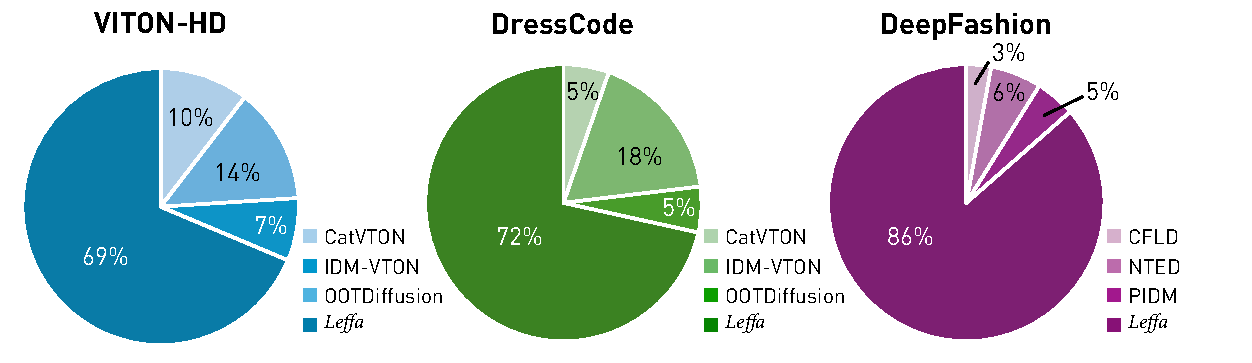
\includegraphics[width=1.0\linewidth]{Chapter6/Figures/human_study_final.pdf}
    \caption{Preference percentage via human studies.
    Our \leffa{} consistently outperforms previous methods across datasets.
    }
    \label{leffa:fig:human_study}
\end{figure}


\subsection{Human Study}
We have observed that some evaluation metrics, such as FID, are highly sensitive to implementation details~\citep{heusel2017gans, kynkaanniemi2022role, peebles2023scalable} and may not accurately reflect image generation quality.
To provide a more comprehensive evaluation, we conduct a human study comparing our \leffa{} with other methods.

Specifically, VITON-HD~\citep{choi2021viton} and DressCode~\citep{morelli2022dress} are selected for virtual try-on , where we compare against OOTDiffusion~\citep{xu2024ootdiffusion}, IDM-VTON~\citep{choi2024improving}, and CatVTON~\citep{chong2024catvton}; while DeepFashion~\citep{liu2016deepfashion} is selected for pose transfer, comparing against PIDM~\citep{bhunia2023person}, NTED~\citep{ren2022neural}, and CFLD~\citep{lu2024coarse}.
We invite 50 participants to evaluate 90 cases (30 randomly selected cases from each dataset), with each participant selecting the image with the best generation quality from each test set.
As shown in Fig.~\ref{leffa:fig:human_study}, our method receives the highest number of preferred selections, significantly outperforming previous methods on both virtual try-on and pose transfer tasks.
